  \let\negmedspace\undefined
\let\negthickspace\undefined
\documentclass[journal]{IEEEtran}
\usepackage[a5paper, margin=10mm, onecolumn]{geometry}
\usepackage{lmodern} % Ensure lmodern is loaded for pdflatex
\usepackage{tfrupee} % Include tfrupee package

\setlength{\headheight}{1cm} % Set the height of the header box
\setlength{\headsep}{0mm}     % Set the distance between the header box and the top of the text

\usepackage{gvv-book}
\usepackage{gvv}
\usepackage{cite}
\usepackage{amsmath,amssymb,amsfonts,amsthm}
\usepackage{algorithmic}
\usepackage{graphicx}
\usepackage{textcomp}
\usepackage{xcolor}
\usepackage{txfonts}
\usepackage{listings}
\usepackage{enumitem}
\usepackage{mathtools}
\usepackage{gensymb}
\usepackage{comment}
\usepackage[breaklinks=true]{hyperref}
\usepackage{tkz-euclide} 
\usepackage{listings}                                      
\def\inputGnumericTable{}                                 
\usepackage[latin1]{inputenc}                                
\usepackage{color}                                            
\usepackage{array}                                            
\usepackage{longtable}
\usepackage{multicol}
\usepackage{calc}                                             
\usepackage{multirow}                                         
\usepackage{hhline}                                           
\usepackage{ifthen}                                           
\usepackage{lscape}
\begin{document}

\bibliographystyle{IEEEtran}
\vspace{3cm}

\title{12.6.5.11}
\author{EE24BTECH11024 - G. Abhimanyu Koushik}
% \maketitle
% \newpage
% \bigskip
{\let\newpage\relax\maketitle}

\renewcommand{\thefigure}{\theenumi}
\renewcommand{\thetable}{\theenumi}
\setlength{\intextsep}{10pt} % Space between text and floats


\numberwithin{equation}{enumi}
\numberwithin{figure}{enumi}
\renewcommand{\thetable}{\theenumi}


\textbf{Question}:\newline
It is given that at $x = 1$, the function $x^4 - 62x^2 + ax + 9$ attains its maximum value, on the interval [0, 2]. Find the value of a.
\newline
\textbf{Solution: }
\newline
Theoritical Solution:\\
Given function
\begin{align}
	f\brak{x} = x^4 - 62x^2 + ax + 9
\end{align}
If a function has a local maxima at $x=x_0$ then $f^\prime\brak{x_0} = 0$ and $f^{\prime\prime}\brak{x_0} \le 0$
\begin{align}
	f^\prime\brak{x} = 4x^3 - 124x + a \\
	f^{\prime\prime}\brak{x} = 12x^2 - 124\\
	f^\prime\brak{1} = 4-124+a\\
	f^{\prime\prime}\brak{1} = 12 - 124\\
\end{align}
$f^{\prime\prime}\brak{1}$ is anyway negative so $f^\prime\brak{1}$ should be $0$
\begin{align}
	a-120 =0\\
	a = 120
\end{align}
When $a = 120$, it satisfies all the conditions.\\
Computational Solution:\\
Given function
\begin{align}
	f\brak{x} = x^4 - 62x^2 + ax + 9
\end{align}
At any critical point $x=x_0$, $\brak{f^\prime\brak{x_0}}^2$ is minimum. We need to minimize
\begin{align}
L\brak{a} = \brak{f^\prime\brak{1}}^2\\
L\brak{a} = \brak{a-120}^2
\end{align}
We use the method of gradient descent to find the minimum of the above function, since the objective function is convex.
\begin{align}
    a_{n+1} &= a_n - \mu L^{\prime}\brak{a_n}\\
    L^{\prime}\brak{a_n} &= 2\brak{a_n-120}\\
    \xrightarrow{} a_{n+1} &= a_n - 2\mu\brak{a_n-120}
\end{align}
Applying unilateral Z-transform,
\begin{align}
    zX\brak{z} - zx_0 &= \brak{1-2\mu}X\brak{z}+\frac{240\mu}{1-z^{-1}}
\end{align}
The Unilateral Z-transform of a constant function $f\brak{x} = c$ is $\frac{c}{1-z^{-1}}$ with Radius of convergence being $\abs{z}>1$
\begin{align}
    \brak{z - \brak{1-2\mu}}X\brak{z} &= zx_0+\frac{240\mu}{1-z^{-1}}\\
    X\brak{z} &= \frac{zx_0}{z - \brak{1-2\mu}}+\frac{240\mu}{\brak{1-z^{-1}}\brak{z - \brak{1-2\mu}}}\\
    X\brak{z} &= \frac{x_0}{1 - \brak{1-2\mu}z^{-1}}+\frac{240\mu}{z-2\brak{1-\mu}+\brak{1-2\mu}z^{-1}}\\
    X\brak{z} &= \frac{x_0}{1 - \brak{1-2\mu}z^{-1}}+\frac{240\mu z^{-1}}{1-2\brak{1-\mu}z^{-1}+\brak{1-2\mu}z^{-2}}\\
    &= \sum_{0}^{\infty} \brak{1-2\mu}^n z^{-n}+\sum_{1}^{\infty}\frac{1-\brak{1-2\mu}^n}{2\mu}z^{-n}\\
    &= \sum_{0}^{\infty} \brak{1-2\mu}^n z^{-n}+\sum_{1}^{\infty}\frac{1}{2\mu}z^{-n}-\sum_{1}^{\infty}\frac{\brak{1-2\mu}^n}{2\mu}z^{-n}\\
\end{align}
From the last equation, ROC is 
\begin{align}
    \abs{z} &> \abs{1-2\mu}\\
    \abs{z} &> 1 \\
    \xrightarrow{} 0 < |1-2\mu| < 1\\
    \xrightarrow{} \mu \in \brak{0, \frac{1}{2}}
\end{align}
Now, if $\mu$ satisfies the previous condition,
\begin{align}
    \lim_{n \to \infty} \brak{a_{n+1} - a_n} = 0\\
    \xrightarrow{} \lim_{n \to \infty} \brak{- 2\mu\brak{a_n-120}} = 0\\
    \xrightarrow{} {-2\mu}\lim_{n \to \infty} \brak{a_n-120} = 0\\
    \xrightarrow{} \lim_{n \to \infty} \brak{a_n} = 120\\
    \xrightarrow{} \lim_{n \to \infty} a_n = 120
\end{align}
Taking initial guess = 50\\ step size = 0.1\\ tolerance(minimum value of gradient) = 1e-5\\ We get \\
$a_{min} = 119.99999528200934$\\
The question minimum value of $L\brak{a} = \brak{a-120}^2$ can be viewed as a Quadratic Programming problem as:\\
\begin{align}
    \min_{\vec{x}} \abs{e_2^{\top}\vec{x}}\\
    \text{s.t. } \\ \vec{x}^{\top}V\vec{x} + 2\vec{u}^{\top}\vec{x} + f = 0\\
    V = \myvec{1 & 0 \\ 0 & 0}\\
    \vec{u} = \myvec{-120 \\ -0.5}\\
    f = 14400
\end{align}
The constraint here is non-convex since the constraint defines a set which is not convex, since points on the
line joining any 2 points on the curve don't belong to the set. However, if we make the constraint
\begin{align}
    \vec{x}^{\top}V\vec{x} + 2\vec{u}^{\top}\vec{x} \le 0
\end{align}
the constraint becomes convex. Using cvxpy to solve this convex optimization problem, we get \\
\begin{align}
    Optimal x: [[ 1.19999997e+02]\\
 [-3.74242669e-05]]
\end{align}
\begin{figure}[h!]
   \centering
   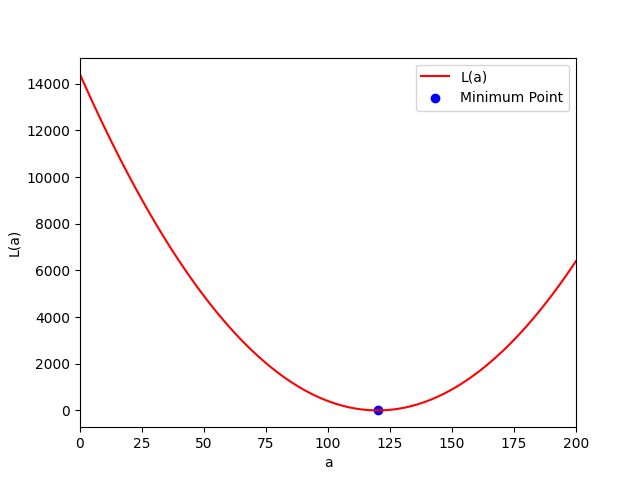
\includegraphics[width=\columnwidth]{figs/fig1.png}
   \caption{Graph of $L\brak{a} = \brak{a - 120}^2$ and the value of $a$ which satisfies the given conditions}
   \label{stemplot}
\end{figure}

\begin{figure}[h!]
   \centering
   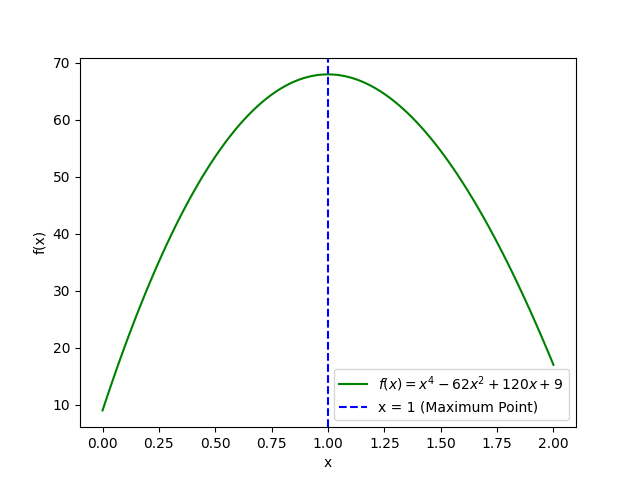
\includegraphics[width=\columnwidth]{figs/fig2.png}
   \caption{Graph of $f\brak{x}$ when $a = 120$}
   \label{stemplot}
\end{figure}
\end{document}  
